\section{Pipeline-Verarbeitung}
\label{sec:pipelining}

\textbf{Pipeline vs Seriell}
\begin{items}
  \item Seriell:
  \begin{figure}[ht]
    \centering
    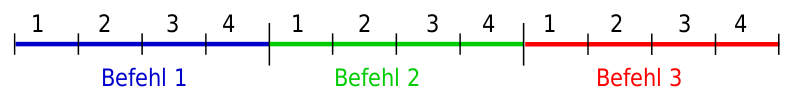
\includegraphics[width=0.33\textwidth]{Seriell}
    \label{Seriell}
  \end{figure}
  \item Pipelining:
  \begin{figure}[ht]
    \centering
    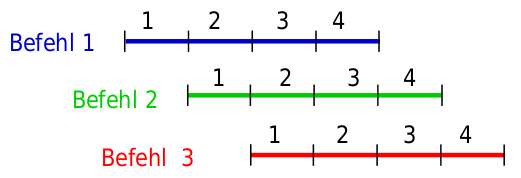
\includegraphics[width=0.33\textwidth]{Pipeline}
    \label{Pipeline}
  \end{figure}
\end{items}

\textbf{Beispiel: Wäsche waschen}
\begin{enumeration}
  \item Schmutzige Wäsche in Waschmaschine
  \item Nasse Wäsche in Trockner
  \item Falten/Bügeln
  \item Kleider in Schrank legen
\end{enumeration}
\begin{figure}[ht]
  \centering
  \label{PipelineWaesche}
  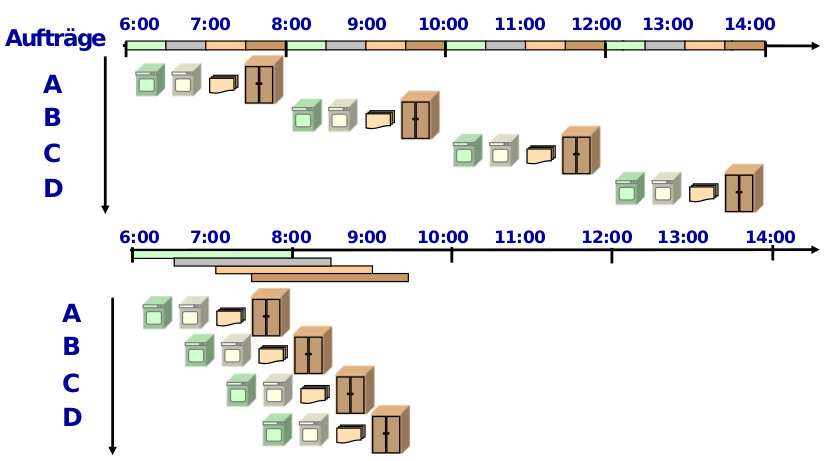
\includegraphics[width=0.33\textwidth]{PipelineWaesche}
\end{figure}

\textbf{Definition} \emph{Pipelining}: Operationszerlegung in mehrere Phasen/Suboperationen, die von hintereinandergeschalteten Verarbeitungseinheiten taktsynchron bearbeitet werden (jede Verarbeitungseinheit führt eine Teiloperation aus). \\*
$\leadsto$ Gesamtheit Verarbeitungseinheiten = Pipeline

\ \\

\textbf{Begrifflichkeiten}
\begin{items}
  \item \underline{Stufen, Register}:
  \begin{figure}[H]
    \centering
    \label{PipelineAufbau}
    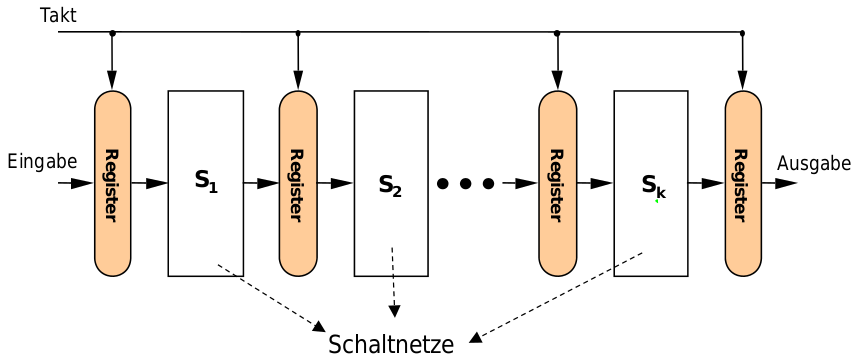
\includegraphics[width=0.33\textwidth]{PipelineAufbau}
  \end{figure}

  \item \underline{Verzögerungszeiten}: Schaltnetze: $\tau_i$ ($i=1,\dots,k$), Register: $\tau_{\text{reg}}$

  \item \underline{Pipeline-Maschinentakt}: Benötigte Zeit, um Befehl eine Stufe weiterzuschieben (ideal: $k$-stufige Pipeline führt Befehl in $k$ Takten mit $k$ Stufen aus)
  \item \underline{Latenz}: Zeit, die ein Befehl braucht, um alle $k$ Stufen zu durchlaufen
  \item \underline{Durchsatz}: Anzahl Befehle, die Pipeline pro Takt verlassen können: $D=\tfrac{n}{(k+n-1)*\tau}$ ($\tau: \text{max}\{ \tau_1,\dots,\tau_k \} + \tau_\text{reg}$) - $\lim_{n \to \infty} D = D_\text{max} = \tfrac{1}{\tau}$
  \item \underline{Speedup}: $n$ Befehle mit $k$-stufiger Pipeline ausführen:
  \begin{enumeration}
    \item sequentiell: $n*k$ Taktzyklen
    \item mit pipelining: $k+(n-1)$ Taktzyklen (Latenz $k$, Durchsatz $1$ - $k$ Takte zum Füllen, $(n-1)$ für die restlichen Befehle)
  \end{enumeration}
  $\leadsto$ Speedup $S=\tfrac{n*k}{k+n-1}$ (Leistungssteigerung - $\lim_{n \to \infty}S=k$)
\end{items}